%%%%%%%%%%%%%%%%%%%%%%%%%%%%%%%%%%%%%%%%%%%%%%%%%%%%%%%%%%%%%%%%%%%%%%%%
%                                                                      %
%     File: Thesis_Results.tex                                         %
%     Tex Master: Thesis.tex                                           %
%                                                                      %
%     Author: Andre C. Marta                                           %
%     Last modified :  2 Jul 2015                                      %
%                                                                      %
%%%%%%%%%%%%%%%%%%%%%%%%%%%%%%%%%%%%%%%%%%%%%%%%%%%%%%%%%%%%%%%%%%%%%%%%

\chapter{Sample generation and analysis tools}
\label{chapter:tools}

A crucial component of this work is the generation of the Monte Carlo samples that are used in the analysis. They are produced using fast simulation. We use the software and machinery that was developed by the FCC study group at CERN. The simulation work flow and Monte Carlo samples are described in this chapter.

In section \ref{sec:workflow} we introduce the generators used to produce the Monte Carlo samples and briefly describe their working principles and functionalities. We then focus on the FCC-hh software, in subsection \ref{subsec:FCC_software}, and explain how the previously described simulation work flow is implemented. A detailed description of the technical settings used to produce the samples is provided in sections \ref{sec:sig+bkg} and \ref{sec:HCALgran}.

%In section \ref{sec:skim}, we briefly mention the skimming procedure we implemented as the first step of the analysis.

\section{Fast simulation workflow}
\label{sec:workflow}

%- Samples used for signal and backgrounds \\
%- Number of events, cross section, how they were generated (gen level cuts)\\

The Monte Carlo samples used in this study were generated using MadGraph5\_aMC@NLO  \cite{MG5}. The showering and hadronization are simulated using Pythia 8 \cite{Pythia8} and the detector response is parametrized using Delphes 3 \cite{Delphes}. These samples are available at the CERN EOS storage. 

MadGraph5 is a matrix element generator for high energy physics processes, such as decays and scatterings. The user specifies the desired process in terms of the initial and final states and can impose additional constraints such as allowing for a number of refined criteria, including forced or forbidden s-channel resonances, excluded internal particles, and forced decay chains of final state particles \cite{MG5}. As a result, MadGraph automatically generates the corresponding Feynman diagrams and creates the necessary code to compute the matrix element at a given point of the phase space. The output file is written in the Les Houches Accord \cite{lhe}.

Pythia8 is frequently used for event generation in high energy physics. In this work, however, we use it only to simulate the showering and hadronization process and not the parton level hard process which is simulated in MadGraph5. The Les Houches file that is produced by MadGraph5 is used as input to a Pythia8 program that can decay unstable particles, simulate initial and final state showers as well as the hadronization of coloured particles, such as quarks and gluons. The desired settings can be specified in an additional file, a card, that is used as input for a Pythia8 run.

Delphes3 allows for a quick and simple simulation of the detector's response \cite{Delphes}. Its goal is to allow the fast simulation of a multipurpose detector for phenomenological studies. The simulation includes a track propagation system, electromagnetic and hadronic calorimeters and a muon identification system. Low level physics objects, such as tracks and energy deposits, and high level physics objects, such as leptons and jets, are reconstructed from the detector's response and can be used to perform physics analysis. In the following paragraphs we briefly describe how the detector response is simulated and how jet reconstruction is performed.  

The magnetic field is uniform, axial and parallel to the beam direction. Charged particles follow a helicoidal trajectory from the interaction point to the calorimeters while neutral particles have a straight line trajectory. The probability of a charged particle being reconstructed as a track is defined by the user. Only a smearing in the modulus of the transverse momentum is applied (not to the direction). The tracking efficiency, as well as energy and momentum resolutions, are specified by the user and may include a dependency on the particle type, momentum and pseudorapidity. The calorimeters have a finite segmentation in the $(\eta,\phi)$ plane and the cell size can be defined in the configuration file. The amount of energy deposited in the calorimeters by each particle type can be defined by the user. By default, stable hadrons deposit all their energy in the HCAL although in a real detector a significant fraction of their energy is deposited in the ECAL. The energy resolution of the ECAL and HCAL are parameterized as a function of $\eta$ and include stochastic, noise and constant terms: $\sigma (E)/E=a/\sqrt{E}\bigoplus b$ . The electromagnetic and hadronic energy deposits are independently smeared by log-normal distributions. 

Jets can be produced using generator level long-lived particles after showering and hadronization, tracks, calorimeter towers or particle-flow tracks and towers. These are referred to as generator, track, calorimeter or particle-flow jets, respectively. For generator level jets no detector simulation nor reconstruction are taken into account. In spite of the type of jet, the user can choose the jet clustering algorithm and the values of its parameters as well as the minimum transverse momentum of the jets that are stored in the final collection. Delphes integrates the FastJet package \cite{fastjet} and therefore allows jet reconstruction with the most popular jet reconstruction algorithms, namely, anti-$k_T$, $k_T$ and Cambridge-Aachen (C/A). 
Jets resulting from the hadronization of a b quark (known as b jets), are identified if a b quark is found within a $\Delta R$ distance from the jet's axis. The tagging efficiency and mis-tagging probabilities can be defined by the user. 

\subsection{Particle flow and calorimeter reconstruction in Delphes}

In Delphes, hadronic jets can be reconstructed using only the information from the HCAL towers or using a particle flow algorithm that combines information from the tracking system and from the HCAL towers. These two approaches create jets that are referred to as calorimeter and particle flow jets, respectively. The latter can also be referred to as energy flow jets (eflow jets in short). In this work we performed the analysis using both sets of jets and compare the results. Therefore we briefly describe them here.

Calorimeter jets are very simple. They are reconstructed using as input for the jet clustering algorithm the 4-vectors associated with the calorimeter towers, after a cell energy smearing has been applied. Therefore the spatial resolution is limited by the transverse segmentation of the calorimeters.

The goal of the particle flow approach is to make use of all the available information provided by the various sub-detectors for reconstructing an event \cite{Delphes}. This approach is used by some experimental collaborations \cite{PF1,PF2} but the exact implementation depends on the specificities of the experiment. If the momentum resolution of the tracking system is better than the energy resolution of the calorimeters it might be convenient to use the tracking information to estimate the momentum of charged particles. In real experiments, the tracking resolution is only better than the calorimeter's energy resolution up to some energy threshold. However, in Delphes, it is assumed that it is always convenient to estimate the momentum of charged particles via the tracker. 

The particle flow algorithm works as follows \cite{Delphes}. For each calorimeter tower it counts:
\begin{itemize}
	\item the total energy deposited in ECAL and HCAL, $E_{\text{ECAL}}$ and $E_{\text{HCAL}}$, respectively;
	\item the total energy deposited in ECAL and HCAL originating from charged particles for which a track has been reconstructed, $E_{\text{ECAL,trk}}$ and $E_{\text{HCAL,trk}}$, respectively.
\end{itemize}
Then it defines $\Delta_{\text{ECAL}}=E_{\text{ECAL}}-E_{\text{ECAL,trk}}$, $\Delta_{\text{HCAL}}=E_{\text{HCAL}}-E_{\text{HCAL,trk}}$ and computes $E^{eflow}_{Tower}$ given by
\begin{equation}
	E^{eflow}_{Tower}=\max(0,\Delta_{\text{ECAL}})+\max(0,\Delta_{\text{HCAL}}).
\end{equation}
All reconstructed tracks result in a particle flow track. If $E^{eflow}_{Tower}>0$ a particle flow tower is created with energy $E^{eflow}_{Tower}$. The particle flow tracks and towers are then used as input for the jet clustering algorithms.

For example \cite{Delphes}, a single charged pion is reconstructed as a track with energy $E_{\text{HCAL,trk}}$
and deposits some energy $E_{HCAL}$ in the hadronic calorimeter. If $E_{\text{HCAL}}\leq E_{\text{HCAL,trk}}$, only a particle flow track with energy $E_{\text{HCAL,trk}}$ is produced. If $E_{\text{HCAL}}>E_{\text{HCAL,trk}}$, a particle flow track with energy $E_{\text{HCAL,trk}}$ and a particle flow tower with energy $E_{\text{HCAL}}$ are produced.

With this algorithm \cite{Delphes}, particle-flow tracks contain charged particles estimated with a
good resolution, while the particle-flow towers contain in general a combination of neutral
particles, charged particles with no corresponding reconstructed track and additional excess
deposits induced by the positive smearing of the calorimeters, and are characterized by a
lower resolution. The particle flow approach produces high resolution inputs for jet clustering algorithms and can also be useful to reduce pileup contributions.

\subsection{FCC-hh software}
\label{subsec:FCC_software}

FCC software (FCCSW) \cite{FCCSW}, common to all FCC studies (electron-electron, electron-hadron and hadron-hadron) has been developed and is maintained by the FCC study group. The software is based on Gaudi \cite{gaudi}. An FCC Event Data Model based on Podio \cite{Podio} was also developed. It consists in specific classes that encode the information about the events.

The FCC-hh study group is responsible for the generation of Monte Carlo quick simulation samples for the main benchmark processes for the FCC-hh and corresponding backgrounds. The samples are generated using the worflow described in the previous section. CERN users can request rights to run the EventProducer package \cite{FCCEventProducer} and produce samples for any desired process using the machinery that is already implemented. In addition, the FCC Event Data Model classes are directly accessible and can be used to read the ROOT files that are produced after the events are passed through Delphes.

The machinery to submit jobs to CERN's batch system is also implemented for both the generation (MadGraph5) and reconstruction (Pythia8 plus Delphes3) levels.

In this work we make use of this software in order to produce the necessary samples.

%\section{Skimming}
%\label{sec:skim}
%
%After the samples are produced, we make use of the FCC Event Data Model classes to read the output ROOT files. We skim through the samples and apply a very loose selection in order to separate the events in three categories: boosted, semi-resolved and resolved. In addition, for the boosted and intermediate categories, that make use of jets with a large R parameter, we also compute the substructure variables. 

\section{Signal and background samples}
\label{sec:sig+bkg}

In this work we focus on the $hh\rightarrow b\overline{b}b\overline{b}$ channel and perform an analysis targeting the boosted kinematic region. The main backgrounds are multijet and $t\overline{t}$ production and the irreducible $pp\rightarrow b\overline{b}b\overline{b}$ process. This was introduced and motivated in chapter \ref{chapter:introduction} and it is discussed in detail in chapter \ref{chapter:analysis}. Here we provide a technical description of how the signal and background samples were generated. 

%The MadGraph5 level cuts are summarized in table \ref{table:MG5cuts}. We show only the most relevant cuts for this analysis: the minimum $p_T$ of light and b quarks, $p_{T,j}^{\min}$ and $p_{T,b}^{\min}$, the maximum pseudorapidity range for light and b quarks, $\eta_j^{\max}$ and $\eta_b^{\max}$ and the $\Delta R$ separation between two light quarks, $\Delta R(jj)$, two b quarks, $\Delta R(bb)$, and between a light and b quarks, $\Delta R(jb)$. The \textit{xqcut} parameter is a measure of the required parton separation at Madgraph level. Whenever MadGraph produces two partons, $i$ and $j$, we define the distance between them as $\sqrt{2*\min{p_{T,i},p_{T,j}}[\cosh{(\eta_i-\eta_j)}-\cos{(\phi_i-\phi_j)}]}$. If the value of this expression is smaller than the specified value of xqcut then we do not generate the event. The \textit{bwcutoff} parameter defines what is considered to be on-shell s-channel resonances. The $H_T$ variable is the scalar sum of the $p_T$ of all truth level partons, including b quarks. 

\subsection{MadGraph}

The irreducible background is generated with an extra jet with a high $p_T$ at generator level, $4b+j$, where $j$ stands for a light jet (initiated by a gluon or $u,d,c,s$ quarks). This is referred to as the four flavor scheme. A high-$p_T$ extra jet forces the four b quarks to have a high Lorentz boost and therefore increases the probability of the events being reconstructed with two large-$R$ jets consistent with a two-prong substructure. For this process, QCD and electroweak contributions are considered separately, i.e, we include three different types of samples: one in which only QCD processes are considered, one in which only electroweak processes are considered and one in which both process are considered simultaneously. The samples do not overlap. The $4b+j$ QCD sample is constituted by two independent samples that have a different generator level cut in the minimum $p_T$ of the light jets, namely, $200<p_{T,j}^{\min}<500$ GeV and $p_{T,j}^{\min}>500$ GeV. This allows for a more efficient generation. 

The multijet background is simulated through $jj+0/1/2 ~j$ where $j$ stands for a light or b jet (five flavor scheme).
This background is divided into several individual samples that are produced in different $H_T$ regions, where $H_T$ is the scalar sum of the $p_T$ of all partons at generator level. The minimum(maximum) allowed $H_T$ is $500(100,000)$ GeV. Since these backgrounds are QCD processes, the $p_T$ distribution of the final state jets falls very steeply as the $p_T$ increases. Therefore, if one were to generate events for these processes without restricting the phase space, most events would consist of jets with a very low $p_T$ which are exactly the type of events that are rejected the most by a boosted analysis (see chapter \ref{chapter:analysis} for more details on the event topology that is targeted and on the analysis strategy). As we move to regions of the phase with a higher $H_T$ the cross section decreases meaning we need fewer MC events to properly simulate the background in that region.

Note that for the $4b+j$ (QCD) and $jj+0/1/2 ~j$ samples we do not take into account the regions of the phase space with $p_{T,j}<200$ GeV and with $0<H_T<500$ GeV. We assume that we can reject most of the events (if not all) with these kinematic characteristics by going to a sufficiently boosted region of the phase space. In addition, note that after the showering procedure there could be some overlap between the $4b+j$ and $jj+0/1/2~ j$. This is taken care of in our analysis code: if an event from the $jj+0/1/2 ~j$ sample has four b quarks at truth level (which happens for approximately $0.01\%$ of the events) then we do not consider it because it will certainly overlap with an event from the $4b+j$ sample.

%The 4b+j is generated using the four flavor scheme meaning that the extra parton can be a gluon or a quark from the first he second geerations. For the jj+0/1/2 j and $t\overline{t}$+0/1/2 j samples the five flavor scheme is used and therefore the extra partons can also be b quarks. Notice that after the showering procedure there could be some overlapp between the 4b+j and jj+0/1/2 j. This is taken care of in our analysis code: if an event from the jj+0/1/2 j has four b quarks at truth level [GIVE PERCENTAGE] then we do not consider it because it will certainly overlapp with an event from the 4b+j sample. 

The $t\overline{t}$ background sample is generated with extra jets at generator level, $t\overline{t}+0/1/2 ~j$, using the five flavor scheme. We consider an inclusive sample for this background, meaning that we do not force any particular decay of the top quark or of the subsequent particles.
 
For the $hh$ SM signal sample, one of the Higgs is decayed to $b\overline{b}$ in MadGraph. The reasoning behind this choice is that most searches for Higgs pair production make use of a final state that includes at least two b quarks in order to keep the cross section times BR of the process large enough. In addition, this method allows the same generator level samples to be used to perform different analysis, simply by choosing the decay channel of the remaining Higgs boson. The decay of the remaining Higgs boson can be implemented in Pythia, in the case of this work, to $b\overline{b}$.

The generator level cuts for the signal and background samples are summarized in table \ref{table:MG5cuts} in appendix \ref{chapter:samples_gen}. 

\subsubsection{Signal samples - BSM} 

In addtion to the SM di-Higgs signal, we also explore the signature and analysis sensitivity for di-Higgs signals produced by two benchmark BSM models: CP-conserving type II 2HDM and a simplified dark matter model (DM) with a spin 0 mediator. These models were described in section \ref{section:BSM}.

Both models are readily available in Feynrules \cite{Feynrules} model database and can be straightforwardly implemented in Madgraph5. The parameters of the models, namely the masses of the new particles, can be changed by the user. In the case of this work, we want new particles to have a large mass so that they produce SM Higgs pairs with a high Lorentz boost. 

%Starting from \cite{2HDMdata}, that constraints the parameter space of the CP-conserving 2HDM using ATLAS and CMS data collected during LHC's $7$ and $8$ TeV runs, we choose values for the masses of the additional Higgs bosons ($h_2$, $h_3$, $h^{\pm}$) that are as high as possible but that are within the allowed (not excluded by experimental data or theoretical constraints) phase space of the model. We set:
%\begin{equation}
%m_{h_2}=600 ~\text{GeV}, \quad m_{h_3}=900 ~\text{GeV}, \quad m_{h^{\pm}}=360. ~\text{GeV}
%\end{equation}
%As a safety check, we test the model with these parameters at a CM energy of $13$ TeV. We obtain a value for the cross section of approximately $0.1$ pb which smaller than the current experimental limit on the cross section.

For the DM model \cite{DM}, the spin 0 mediator's mass is set at $1$ TeV. The cross section for the signal generated with this model is smaller than the cross section of the SM signal (approximately $0.2$ pb \textit{versus} $0.7$ pb) and therefore this model is not excluded by experimental data.

For the 2HDM \cite{2HDM,2HDM1}, a finer tuning of the parameters is required because the model is very general and has many free parameters. In addition, it is written in the Higgs basis such that we need to convert the parameters from the physical basis (introduced in section \ref{section:BSM}) to this basis. The free parameters of the model are the masses of the neutral, $m_{h_1}, m_{h_2}, m_{h_3}$, and charged scalars, $m_{hc}$, the neutral scalars mixing angles, $mix_h, mix_{h_2}, mix_{h_3}$, the real and imaginary parts of the up, down and charged lepton $3\times 3$ Yukawa matrices, $GUR, GUI, GDR, GDI, GLR, GLI$ and the values (real and imaginary parts) of the second, third and seventh quartic couplings, $l_{2,3,7}$,. In the CP-conserving model $h_{1,2,3}$ can be identified with the physical states $h$, $H$ and $A$, respectively.

We start from the following parameters (in the physical basis):
\begin{align}
	&m_h=125 ~\text{GeV}, \quad m_H=900 ~\text{GeV},\quad m_A=850 ~\text{GeV}, \quad m_{H^{\pm}}=800 ~\text{GeV} \nonumber \\
	&\beta=\frac{\pi}{4}, \quad \alpha = -0.75\nonumber \\	 
	&m_{12}^2=[(m_H^2+m_A^2+m_{H^{\pm}}^2)/3] \cos(\beta)\sin(\beta)\simeq181041.6667.
	\label{eq:2HDMphys_par}
\end{align}
In the Higgs basis, the input parameters for the model are
\begin{align}
&m_{h_1}=125 ~\text{GeV}, \quad m_{h_2}=900 ~\text{GeV},\quad m_{h_3}=850 ~\text{GeV}, \quad m_{hc}=800 ~\text{GeV} \nonumber \\
&mix_{h_2}=mix_{h_3} =0 \nonumber \\
&mix_{h_1}=\frac{\pi}{2}-(\beta-\alpha)\simeq 0.035 \nonumber \\
&l_2\simeq 0.27, \quad l_3\simeq 9.46, \quad l_7\simeq 0.46.
\label{eq:2HDMhiggs_par}
\end{align}
The masses of the scalars cannot change when going from one basis to the other. Therefore we set them to the exact same values. $mix_{h_2},mix_{h_3}=0$ because we are considering the CP-conserving model.
To obtain the values of $l_{2,3,7}$ we use Eq. 11 from Ref. \cite{2HDMpedro} and write the $\lambda$ parameters of the scalar potential in terms of the parameters defined in Eq. \ref{eq:2HDMphys_par}. Then we use Eq. 47,48 and 50 from Ref. \cite{2HDMhaber} to obtain the values of the quartic coupling in the Higgs basis.

Regarding the Yukawa interactions, we work in the type II model. Following the type II restriction file found in Ref. \cite{2HDM} we set
\begin{align}
	&GLR=GLI=GDI=GUI=0 \nonumber \\
	&GDR=\text{diag}\left(0,0,\frac{m_b\sqrt{2}\tan(\beta)}{v}\right) \nonumber \\
	&GUR=\text{diag}\left(0,0,-\frac{m_t\sqrt{2}}{v\tan(\beta)}\right)
\end{align}	
where $m_b=4.7$ GeV and $m_t=172$ GeV are the masses of the bottom and top quarks.

\subsection{Pythia}
\label{sec:Pythia_samples}

For the signal samples (SM and BSM) we simply turn off all other decays except $h\rightarrow b\overline{b}$ therefore forcing the Higgs to decay to a pair of b quarks leading to the desired final state with four b quarks. All other settings are not altered with respect to their default configuration. For the BSM samples, this implies that the coupling of the SM Higgs boson to the b quarks is set to its SM value.

For the $jj+0/1/2 ~$ and $t\overline{t}+0/1/2 ~j$ samples we have to perform jet matching because we require additional jets at the level of the matrix element. In addition to the partons generated in MadGraph and that can produce a jet, Pythia may introduce extra jets that are usually soft and collinear (with the particle from which they were radiated) and result from the showering process. This could lead to the same process (with the same final states) being counted twice (double counting). Take, for example, the processes $j~j$ and  $j~j~j$ at MadGraph level. It can happen that Pythia generates an extra jet for the first process but not for the second, leading to both processes having the same final state (three jets). Each process would then give its independent contribution to the total number of events but because they simply represent two distinct ways of achieving the same final state they should only be counted once. The goal of jet matching procedures is to avoid this problem. 

%The settings for jet matching can be found in table \ref{table:Pythia8settings} under the corresponding samples' columns. We perform the jet matching procedure (merge=on) using the MLM matching scheme and the appropriate algorithm for a parton level process generated in MadGraph (scheme=1). We do not read the matching parameters from the MadGraph file (setMad=off) because this option is not available for these files. The size of the cone drawn around the jet's center, the maximum pseudorapidity and the maximum number of jets to be matched are given by coneRadius, etaJetMax and nJetMax, respectively. The cone radius is set to one. The maximum allowed pseudorapidity of jets is ten which is a much loser cut than the acceptance of any current detector. The maximum number of jets is set to four for the jj+0/1/2 j and to two for the $t\overline{t}$+0/1/2 j. The qCut parameter defines the $k_T$ scale for merging shower products into jets.  

The cross section times branching ratio (when applicable), the k-factors and the approximate number of events for the samples used in the analysis are summarized in table \ref{table:samples_summary}. The k-factor multiplies the cross section times branching ratio in order to reproduce known higher order results. It corresponds only to the ratio between the total cross sections and it does not correct for possible differences that might exist between the differential cross sections. The number of events changes according to the granularity configuration and to the type of jets that were used. The numbers shown should be taken only as an order of magnitude.

For the SM signal, $\sigma\times BR$ is given by $\sigma(hh,h\rightarrow b\overline{b})\times BR(h\rightarrow b\overline{b})$, with $BR(h\rightarrow b\overline{b})=0.5824$ for $m_h=125$ GeV \cite{HiggsHandbook}. $\sigma(hh,h\rightarrow b\overline{b})$ is given by:
\begin{equation}
	\sigma(hh,h\rightarrow b\overline{b})=\sigma_{NNLO}(hh)\times 2\times BR(h\rightarrow b\overline{b})=1.22~\text{pb}\times 2 \times 0.5824 = 1.42 ~\text{pb}
\end{equation}
where $\sigma_{NNLO}(hh)=1.22$ pb follows from Ref. \cite{HxsNNLO} and the factor of $2$ is a combinatorial factor that indicates that both Higgs bosons can decay to a pair of b quarks. The k-factor is given by $\sigma_{\text{NNLL}}/\sigma_{\text{NNLO}}$, where $\sigma_{\text{NNLL}}$ is calculated according to the prescription given in equation I.7.8 of Ref. \cite{HiggsHandbook}, with $\delta_t=-0.315$, which yields $\sigma_{\text{NNLL}}=1.33$ pb. Therefore, the k-factor has the value $1.09$.

For the BSM signal samples, $\sigma\times BR$ is given by:
\begin{equation}
	\sigma\times BR = \sigma(hh)_{\text{MG}}\times (BR(h\rightarrow b\overline{b}))^2
\end{equation}
where $\sigma(hh)_{\text{MG}}$ is the cross section for Higgs pair production as given by MadGraph. For these samples we consider a k-factor of $1.0$.

For the remaining samples, $\sigma\times BR$ are the values given by MadGraph. In these samples no decay mode is imposed, therefore the branching ratio is one. For the $4b+j$(QCD) samples, a k-factor of two is applied \cite{FCCEventProducer} in order to parameterize our ignorance on the QCD irreducible background. For the $t\overline{t}+0/1/2 ~j$, a k-factor of $1.74$ is applied, following Ref. \cite{FCCEventProducer}.

The parameters used in Pyhtia 8 can be found in table \ref{table:Pythia8settings} in appendix \ref{chapter:samples_gen}.

\begin{table}
	\centering
	\caption{Summary of the effective cross sections ($\sigma\times BR$) and k factors of the signal and background samples used in the analysis.}
	\begin{tabular}{llll}
		\toprule 
		\textbf{Sample} & $\sigma\times BR$ [pb] & k-factor & $\sim$ no. events \\
		\midrule
		$hh\rightarrow b\overline{b}b\overline{b}$ - \textbf{SM} & $0.827$ & $1.09$ & $5\times 10^6$\\
		\rowcolor{black!7} $hh\rightarrow b\overline{b}b\overline{b}$ - \textbf{DM mediator} & $0.218$ & $1.0$ & $5\times 10^6$\\
		$hh\rightarrow b\overline{b}b\overline{b}$ - \textbf{2HDM type II} & $0.466$ & $1.0$ & $5\times 10^6$\\
		\rowcolor{black!7} $4b+j$ (QCD, $200<p_T^j<500$)& $756.4$ & $2.0$ & $10\times 10^6$\\
		$4b+j$ (QCD, $p_T^j>500$)& $57.71$ & $2.0$ & $10\times 10^6$\\
		\rowcolor{black!7}$4b+j$ (QCD+EWK) & $6.204$ & $1.0$ & $10\times 10^6$\\
		$4b+j$ (EWK)& $0.07206$ & $1.0$ & $5\times 10^6$\\
		\rowcolor{black!7} $jj+0/1/2 ~j$ ($500<H_T<1000$) & $1.64\times 10^7$ &$1.0$&$10\times 10^6$\\
		$jj+0/1/2 ~j$ ($1000<H_T<2000$) & $1.67\times 10^6$ &$1.0$ & $1\times 10^6$\\
		\rowcolor{black!7}$jj+0/1/2 ~j$ ($2000<H_T<4000$) & $1.32\times 10^5$ & $1.0$&$1\times 10^6$\\
		$jj+0/1/2 ~j$ ($4000<H_T<7200$) & $7.32\times 10^3$ & $1.0$&$1\times 10^6$\\
		\rowcolor{black!7}$jj+0/1/2 ~j$ ($7200<H_T<15000$) & $4.75\times 10^2$ & $1.0$&$1\times 10^6$\\
		$jj+0/1/2 ~j$ ($15000<H_T<25000$) & $7.35$ & $1.0$&$1\times 10^6$\\
		\rowcolor{black!7}$jj+0/1/2 ~j$ ($25000<H_T<35000$) & $0.176$ & $1.0$&$5\times 10^5$\\
		$jj+0/1/2 ~j$ ($35000<H_T<100000$) & $0.00765$ & $1.0$&$3\times 10^5$\\
		\rowcolor{black!7}$t\overline{t}+0/1/2 ~j$ & $4.31	\times 10^4$ & $1.74$ &$5\times 10^6$\\
		\bottomrule
	\end{tabular}
	\label{table:samples_summary}
\end{table}

\subsection{Delphes}
\label{sec:HCALgran}

It is one of the main goals of this work to evaluate how the analysis sensitivity is influenced by the granularity of the hadronic calorimeter. We start from the same MadGraph level samples and pass them through Pythia and Delphes changing the settings of the Delphes card that correspond to the HCAL. All other detector's parameters were kept unchanged with respect to the FCC default Delphes card. 
We tested five benchmark granularity configurations:

\begin{enumerate}
	\item ATLAS HCAL granularity (as implemented in the standard ATLAS Delphes card);
	\item Starting from the ATLAS HCAL configuration we increase the granularity in $\eta$ by a factor of four, in the pseudo rapidity range $|\eta|<1.7$ which corresponds to the TileCal region;
	\item Starting from the FCC HCAL configuration we decrease the granularity in $\phi$ by a factor of two, in the entire pseudo rapidity range covered by the HCAL.
	\item FCC HCAL default granularity (as implemented in the standard FCC Delphes card);
	\item Starting from the FCC HCAL configuration we increase the granularity in $\eta$ and in $\phi$ by a factor of two, in the entire pseudo rapidity range covered by the HCAL.
\end{enumerate}

The granularities of these five configurations are summarized in table \ref{table:Gran}. The values that are shown, as well as the corresponding pseudorapidity regions, are exactly what is implemented in Delphes. 

In addition, we also passed the same generator level samples through the default ATLAS detector simulation in Delphes. The HCAL granularity is the one that is indicated in the second row of table \ref{table:Gran} but the other detector parameters, such as the radius, magnetic field, tracking resolutions are the ones that are implemented in the default ATLAS Delphes card. This additional detector configuration gives us an extra point in the space of parameters that we are trying to explore. Furthermore, in a first, very crude, approximation, it allow us to compare the results obtained at $\sqrt{s}=100$ TeV to the ones obtained at $\sqrt{s}=13$ TeV by ATLAS.
For completion we summarize, in table \ref{table:det}, the values of some key detector parameters as implemented in Delphes for the ATLAS and FCC-hh detectors. The magnetic field is twice as strong for the FCC-hh. The charged hadrons tracking efficiency and the HCAL resolution are fairly similar between the two detector configurations.

\begin{table}
	\centering
	\caption{Summary of the benchmark granularity configurations of the HCAL.}
	\begin{tabular}{lll}
		\toprule 
		\textbf{Configuration} & $\Delta \eta \times \Delta \phi$ & $\eta$ range\\
		\midrule
		\multirow{2}{*}{1 (ATLAS HCAL)} & $0.1\times 0.1$  & $|\eta|<2.5$\\
		& $0.2\times 0.2$ & $2.5<|\eta|<5.0$ \\
		\cellcolor{black!7} &\cellcolor{black!7} $0.025\times 0.1$  & \cellcolor{black!7}$|\eta|<1.7$\\
		\cellcolor{black!7} & \cellcolor{black!7}$0.1\times 0.1$  & \cellcolor{black!7}$1.7<|\eta|<2.5$\\
		\multirow{-3}{*}{2 (ATLAS HCAL $\eta\times 4$)} \cellcolor{black!7}& \cellcolor{black!7}$0.2\times 0.2$  &\cellcolor{black!7} $2.5<|\eta|<5.0$\\
		\multirow{2}{*}{3 (FCC HCAL $\phi/2 $)}& $0.025\times0.05$ & $|\eta|<2.5$\\
		& $0.05\times 0.1$ & $2.5<|\eta|<6.0$ \\
		 \cellcolor{black!7}&  \cellcolor{black!7}$0.025\times0.025$ &  \cellcolor{black!7}$|\eta|<2.5$\\
		 \multirow{-2}{*}{4 (FCC HCAL)}\cellcolor{black!7}&  \cellcolor{black!7}$0.05\times 0.05$ & \cellcolor{black!7} $2.5<|\eta|<6.0$ \\
		& $0.0125\times0.0125$ &$|\eta|<2.5$\\
		\multirow{-2}{*}{5 (FCC HCAL $\eta,\phi\times 2$)}&$0.025\times 0.025$ & $2.5<|\eta|<6.0$\\
		\bottomrule
	\end{tabular}
	\label{table:Gran}
\end{table}

\begin{table}
	\centering
	\caption{Summary of some key detector parameters for the FCC-hh and ATLAS detectors.}
	\begin{tabular}{p{40mm}p{40mm}p{40mm}}
		\toprule 
		\textbf{Parameter} & FCC-hh & ATLAS\\
		\midrule
		Radius of magnetic field coverage [m]& $1.5$& $1.15$  \\
		\cellcolor{black!7}Half length [m] &\cellcolor{black!7} $5$&\cellcolor{black!7} $3.51$\\
		Magnetic field [T]& $4$& $2$\\
		\cellcolor{black!7}Charged hadrons tracking efficiency &\cellcolor{black!7} $90\%$ for $2.5<|\eta|<4.0$,\linebreak$ p_T>1.0$&\cellcolor{black!7} $85\%$ for $1.5<|\eta|<2.5$,\linebreak$p_T>1.0$\\
		HCAL resolution & $\sqrt{E^2(0.03)^2+E(0.60)^2}$\linebreak for $1.7<|\eta|<4.0$& $\sqrt{E^2(0.05)^2+E(0.706)^2}$ \linebreak for $1.7<|\eta|<3.2$\\
		\bottomrule
	\end{tabular}
	\label{table:det}
\end{table}

%\begin{figure}[!htb]
%  \centering
%  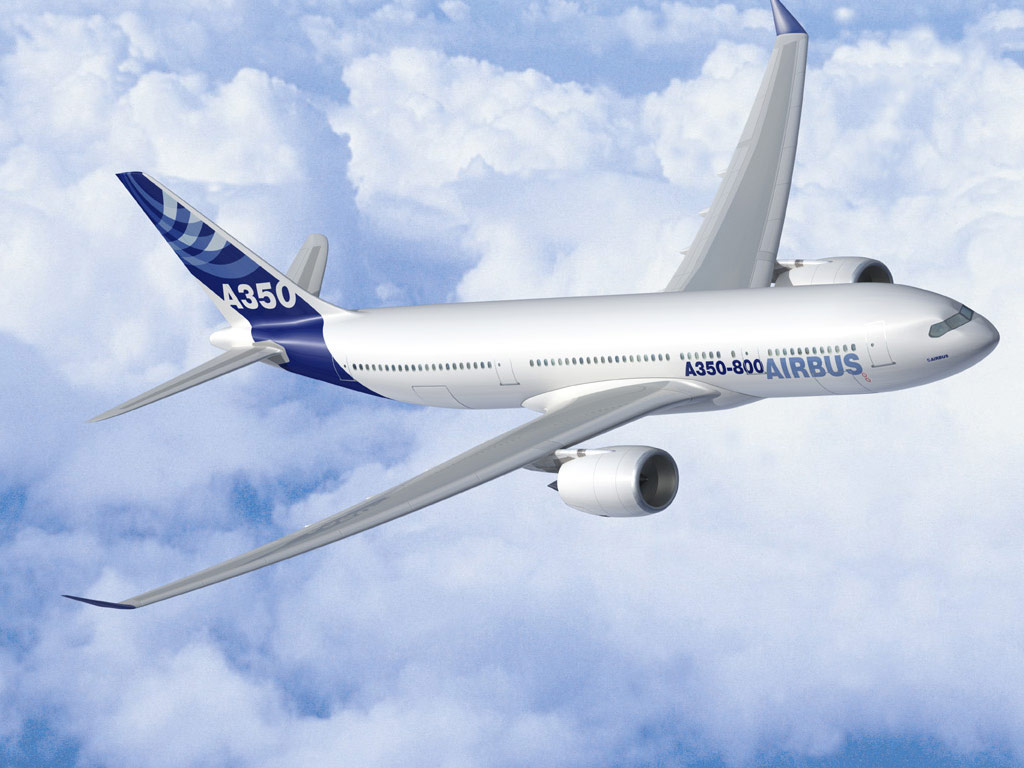
\includegraphics[width=0.25\textwidth]{Figures/Airbus_A350.jpg}
%  \caption[Caption for figure in TOC.]{Caption for figure.}
%  \label{fig:airbus1}
%\end{figure}
%
%\begin{figure}[!htb]
%  \begin{subfigmatrix}{2}
%    \subfigure[Airbus A320]{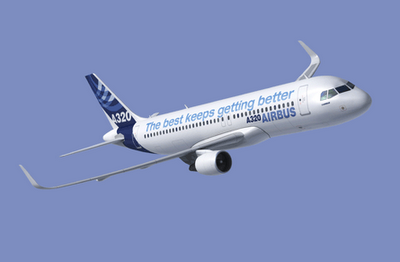
\includegraphics[width=0.49\linewidth]{Figures/Airbus_A320_sharklets.png}}
%    \subfigure[Bombardier CRJ200]{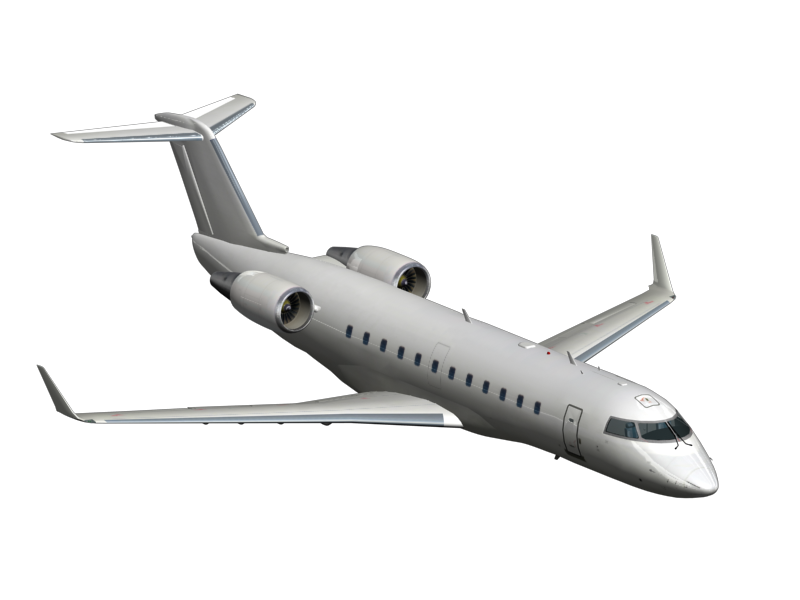
\includegraphics[width=0.49\linewidth]{Figures/Bombardier_CRJ200.png}}
%  \end{subfigmatrix}
%  \caption{Some aircrafts.}
%  \label{fig:aircrafts}
%\end{figure}
%
%Make reference to Figures \ref{fig:airbus1} and \ref{fig:aircrafts}.
%
%By default, the supported file types are {\it .png,.pdf,.jpg,.mps,.jpeg,.PNG,.PDF,.JPG,.JPEG}.
%
%See \url{http://mactex-wiki.tug.org/wiki/index.php/Graphics_inclusion} for adding support to other extensions.
%
%
%% ----------------------------------------------------------------------
%\subsubsection{Drawings}
%\label{subsection:drawings}
%
%Insert your subsection material and for instance a few drawings...
%
%The schematic illustrated in Fig.~\ref{fig:algorithm} can represent some sort of algorithm.
%
%\begin{figure}[!htb]
%  \centering
%  \scriptsize
%%  \footnotesize 
%%  \small
%  \setlength{\unitlength}{0.9cm}
%  \begin{picture}(8.5,6)
%    \linethickness{0.3mm}
%
%    \put(3,6){\vector(0,-1){1}}
%    \put(3.5,5.4){$\bf \alpha$}
%    \put(3,4.5){\oval(6,1){}}
%    %\put(0,4){\framebox(6,1){}}
%    \put(0.3,4.4){Grid Generation: \quad ${\bf x} = {\bf x}\left({\bf \alpha}\right)$}
%
%    \put(3,4){\vector(0,-1){1}}
%    \put(3.5,3.4){$\bf x$}
%    \put(3,2.5){\oval(6,1){}}
%    %\put(0,2){\framebox(6,1){}}
%    \put(0.3,2.4){Flow Solver: \quad ${\cal R}\left({\bf x},{\bf q}\left({\bf x}\right)\right) = 0$}
%
%    \put(6.0,2.5){\vector(1,0){1}}
%    \put(6.4,3){$Y_1$}
%
%    \put(3,2){\vector(0,-1){1}}
%    \put(3.5,1.4){$\bf q$}
%    \put(3,0.5){\oval(6,1){}}
%    %\put(0,0){\framebox(6,1){}}
%    \put(0.3,0.4){Structural Solver: \quad ${\cal M}\left({\bf x},{\bf q}\left({\bf x}\right)\right) = 0$}
%
%    \put(6.0,0.5){\vector(1,0){1}}
%    \put(6.4,1){$Y_2$}
%
%    %\put(7.8,2.5){\oval(1.6,5){}}
%    \put(7.0,0){\framebox(1.6,5){}}
%    \put(7.1,2.5){Optimizer}
%    \put(7.8,5){\line(0,1){1}}
%    \put(7.8,6){\line(-1,0){4.8}}
%  \end{picture}
%  \caption{Schematic of some algorithm.}
%  \label{fig:algorithm}
%\end{figure}
%
%
%% ----------------------------------------------------------------------
%\subsection{Equations}
%\label{subsection:equations}
%
%Equations can be inserted in different ways.
%
%The simplest way is in a separate line like this
%
%\begin{equation}
%  \frac{{\rm d} q_{ijk}}{{\rm d} t} + {\cal R}_{ijk}({\bf q}) = 0 \,.
%\label{eq:ode}
%\end{equation}
%
%If the equation is to be embedded in the text. One can do it like this ${\partial {\cal R}}/{\partial {\bf q}}=0$.
%
%It may also be split in different lines like this
%
%\begin{eqnarray}
%  {\rm Minimize}   && Y({\bf \alpha},{\bf q}({\bf \alpha}))            \nonumber           \\
%  {\rm w.r.t.}     && {\bf \alpha} \,,                                 \label{eq:minimize} \\
%  {\rm subject~to} && {\cal R}({\bf \alpha},{\bf q}({\bf \alpha})) = 0 \nonumber           \\
%                   &&       C ({\bf \alpha},{\bf q}({\bf \alpha})) = 0 \,. \nonumber
%\end{eqnarray}
%
%It is also possible to use subequations. Equations~\ref{eq:continuity}, \ref{eq:momentum} and \ref{eq:energy} form the Naver--Stokes equations~\ref{eq:NavierStokes}.
%
%\begin{subequations}
%    \begin{equation}
%    \frac{\partial \rho}{\partial t} + \frac{\partial}{\partial x_j}\left( \rho u_j \right) = 0 \,,
%    \label{eq:continuity}
%    \end{equation}
%    \begin{equation}
%    \frac{\partial}{\partial t}\left( \rho u_i \right) + \frac{\partial}{\partial x_j} \left( \rho u_i u_j + p \delta_{ij} - \tau_{ji} \right) = 0, \quad i=1,2,3 \,,
%    \label{eq:momentum}
%    \end{equation}
%    \begin{equation}
%        \frac{\partial}{\partial t}\left( \rho E \right) + \frac{\partial}{\partial x_j} \left( \rho E u_j + p u_j - u_i \tau_{ij} + q_j \right) = 0 \,.
%    \label{eq:energy}
%    \end{equation}
%\label{eq:NavierStokes}%
%\end{subequations}
%
%
%% ----------------------------------------------------------------------
%\subsection{Tables}
%\label{section:tables}
%
%Insert your subsection material and for instance a few tables...
%
%Make sure all tables presented are referenced in the text!
%
%Follow some guidelines when making tables:
%
%\begin{itemize}
%  \item Avoid vertical lines
%  \item Avoid “boxing up” cells, usually 3 horizontal lines are enough: above, below, and after heading
%  \item Avoid double horizontal lines
%  \item Add enough space between rows
%\end{itemize}
%
%\begin{table}[!htb]
%  \renewcommand{\arraystretch}{1.2} % more space between rows
%  \centering
%  \begin{tabular}{lccc}
%    \toprule
%    Model           & $C_L$ & $C_D$ & $C_{M y}$ \\
%    \midrule
%    Euler           & 0.083 & 0.021 & -0.110    \\
%    Navier--Stokes  & 0.078 & 0.023 & -0.101    \\
%    \bottomrule
%  \end{tabular}
%  \caption[Table caption shown in TOC.]{Table caption.}
%  \label{tab:aeroCoeff}
%\end{table}
%
%Make reference to Table \ref{tab:aeroCoeff}.
%
%Tables \ref{tab:memory} and \ref{tab:multipleColumns} are examples of tables with merging columns:
%
%\begin{table}[!htb]
%  \renewcommand{\arraystretch}{1.2} % more space between rows
%  \centering
%  \begin{tabular}[]{lrr}
%    \toprule
%                & \multicolumn{2}{c}{\underline{Virtual memory [MB]}} \\
%                & Euler       & Navier--Stokes \\
%    \midrule
%      Wing only &  1,000      &    2,000       \\
%      Aircraft  &  5,000      &   10,000       \\
%      (ratio)   & $5.0\times$ & $5.0\times$    \\
%    \bottomrule
%  \end{tabular}
%  \caption{Memory usage comparison (in MB).}
%  \label{tab:memory}
%\end{table}
%
%\begin{table}[!htb]
%  \centering
%  \renewcommand{\arraystretch}{1.2} % more space between rows
%  \begin{tabular}{@{}rrrrcrrr@{}} % remove space to the vertical edges @{}...@{}
%    \toprule
%      & \multicolumn{3}{c}{$w = 2$} & \phantom{abc} & \multicolumn{3}{c}{$w = 4$} \\
%    \cmidrule{2-4}
%    \cmidrule{6-8}
%      & $t=0$ & $t=1$ & $t=2$ && $t=0$ & $t=1$ & $t=2$ \\
%    \midrule
%      $dir=1$
%      \\
%      $c$ &  0.07 &  0.16 &  0.29 &&  0.36 &  0.71 &   3.18 \\
%      $c$ & -0.86 & 50.04 &  5.93 && -9.07 & 29.09 &  46.21 \\
%      $c$ & 14.27 &-50.96 &-14.27 && 12.22 &-63.54 &-381.09 \\
%      $dir=0$
%      \\
%      $c$ &  0.03 &  1.24 &  0.21 &&  0.35 & -0.27 &  2.14 \\
%      $c$ &-17.90 &-37.11 &  8.85 &&-30.73 & -9.59 & -3.00 \\
%      $c$ &105.55 & 23.11 &-94.73 &&100.24 & 41.27 &-25.73 \\
%    \bottomrule
%  \end{tabular}
%  \caption{Another table caption.}
%  \label{tab:multipleColumns}
%\end{table}
%
%An example with merging rows can be seen in Tab.\ref{tab:multipleRows}.
%
%\begin{table}[!htb]
%  \renewcommand{\arraystretch}{1.2} % more space between rows
%  \centering
%  \begin{tabular}{ccccc}
%    \toprule
%      \multirow{2}{*}{ABC} & \multicolumn{4}{c}{header} \\
%      \cmidrule{2-5} & 1.1 & 2.2 & 3.3 & 4.4 \\
%    \midrule
%      \multirow{2}{*}{IJK} & \multicolumn{2}{c}{\multirow{2}{*}{group}} & 0.5 & 0.6 \\
%      \cmidrule{4-5}       & \multicolumn{2}{c}{}                       & 0.7 & 1.2 \\
%    \bottomrule
%  \end{tabular}
%  \caption{Yet another table caption.}
%  \label{tab:multipleRows}
%\end{table}
%
%If the table has too many columns, it can be scaled to fit the text widht, as in Tab.\ref{tab:scale}.
%\begin{table}[!htb]
%  \renewcommand{\arraystretch}{1.2} % more space between rows
%  \centering
%  \resizebox*{\textwidth}{!}{%
%    \begin{tabular}[]{lcccccccccc}
%      \toprule
%        Variable &  a  &  b  &  c  &  d  &  e  &  f  &  g  &  h  &  i  &  j  \\
%      \midrule
%        Test 1   &  10,000 &  20,000 &  30,000 &  40,000 &  50,000 &  60,000 &  70,000 &  80,000 &  90,000 & 100,000 \\
%        Test 2   &  20,000 &  40,000 &  60,000 &  80,000 & 100,000 & 120,000 & 140,000 & 160,000 & 180,000 & 200,000 \\
%      \bottomrule
%    \end{tabular}
%  }%
%  \caption{Very wide table.}
%  \label{tab:scale}%
%\end{table}
%
%
%% ----------------------------------------------------------------------
%\subsection{Mixing}
%\label{section:mixing}
%
%If necessary, a figure and a table can be put side-by-side as in Fig.\ref{fig:side_by_side}
%
%\begin{figure}[!htb]
%  \begin{minipage}[b]{0.60\linewidth}
%    \centering
%    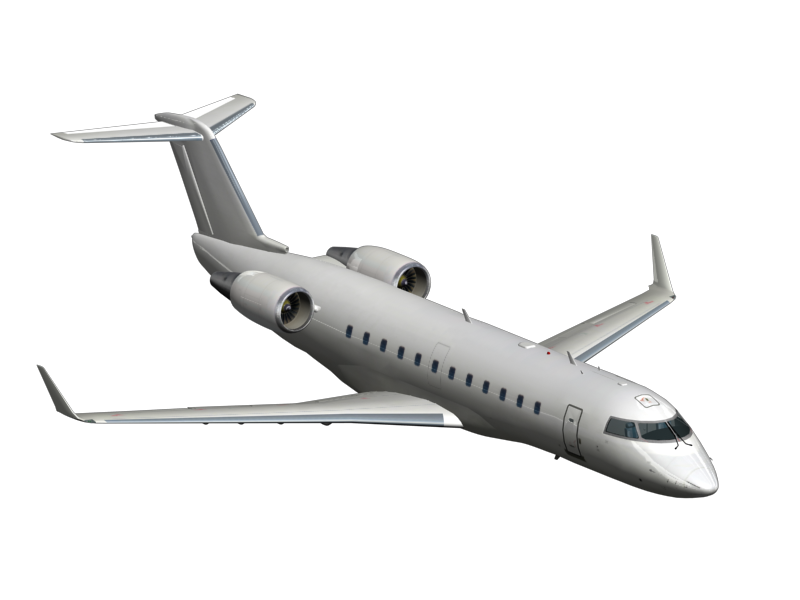
\includegraphics[width=\linewidth]{Figures/Bombardier_CRJ200}
%  \end{minipage}%
%  \begin{minipage}[b]{0.30\linewidth}
%    \centering
%    \begin{tabular}[b]{lll}
%      \toprule
%        \multicolumn{3}{c}{Legend} \\
%      \midrule
%        A & B & C \\
%        0 & 0 & 0 \\
%        0 & 1 & 0 \\
%        1 & 0 & 0 \\
%        1 & 1 & 1 \\
%      \bottomrule
%    \end{tabular}
%    \vspace{5em}
%  \end{minipage}
%\caption{Figure and table side-by-side.}
%\label{fig:side_by_side}
%\end{figure}

